\section{Global Fit Stability}
%\label{sec:globalFitStability} % uncomment if label used. 
\subsection{Signal Injection}
%\label{subsec:globalFitStability:SignalInjection} % uncomment if label used. 
Since to produce the background fit our full signal range is fitted, if our signal region contains a signal our background fit will be modified compared to the case where the signal region is purely background, referred to as the fit stability. As the dijet fit functions are motivated by theory for the QCD dijet distribution, in particular that they are smooth and monotonically decreasing, the effect on the fit should be negligible when injecting a signal with a width small compared to the full fit range. However, it is important to verify that this is the case.

To measure the effect of signal contamination on our background fit, the following method has been used:

\begin{itemize}
    \item Take nominal background fit from fitting data with 5param dijet function.
    \item Add signal to nominal fit to get signal+background fit.
    \item Generate 1,000 pseudoexperiments from signal+background fit.
    \item Loop over every pseudoexperiment:
    \begin{itemize}
        \item generate new background fit (bkg$_{PE}$ from pseudoexperiment).
        \item calculate excess events per bin by subtracting bkg$_{PE}$.
    \end{itemize}
    \item Get average \& standard deviation of all pseudoexperiments excess events per bin.
    \item Look at bins around resonance ('around' chosen such that $\approx$50\% of the total events in the signal are considered, $\approx$ rather than exact since the bins are quite wide \& signal falls rapidly. This roughly corresponds to the region found by BumpHunter at $\approx$3$\sigma$).
    \item Compare excess events in bins around resonance to injected events. (Importantly, retrieved events \& injected events are the retrieved \& injected events in this region around resonance, not over full fit).
    \item Do same with subtracting nominal fit instead of new fit to compare.
\end{itemize}

A table showing how many injected events correspond to a BumpHunter significance of 1, 2 and 3 $\sigma$ is shown in Table \ref{tab:BHSignifcanceStringInjection} to help determine how significant a signal must be injected before the effect of the fit stability is relevant. The results for number of average retrieved events for an injected number of signal events  for a 7.0, 7.5, 8.0, 8.5 and 9.0 TeV string signal injections are shown in Figures \ref{fig:StringSignalInjectionFitStabilityStudyMs7.0TeV}-\ref{fig:StringSignalInjectionFitStabilityStudyMs9.0TeV} respectively. 

\begin{table}[]
    \tiny
    \begin{center}
%        \hspace*{-4cm}
        \begin{tabular}{l|lll|lll|lll|lll|lll|}
            \toprule
            \midrule
            String Scale {[}TeV{]}   & \multicolumn{3}{c|}{7.0}             & \multicolumn{3}{c|}{7.5}             &
\multicolumn{3}{c|}{8.0}             & \multicolumn{3}{c|}{8.5}             & \multicolumn{3}{c|}{9.0}             \\
            \midrule
            Resonance Bins {[}GeV{]} & \multicolumn{3}{c|}{{[}6047-7188{]}} & \multicolumn{3}{c|}{{[}6407-7610{]}} & \multicolumn{3}{c|}{{[}6918-8208{]}} & \multicolumn{3}{c|}{{[}7326-8685{]}} & \multicolumn{3}{c|}{{[}7756-9191{]}} \\
            Bumphunter Significance  & 1          & 2          & 3          & 1          & 2          & 3          & 1          & 2          & 3          & 1          & 2          & 3          & 1          & 2          & 3          \\
            Injected Events          & 23.95      & 34.35      & 44.36      & 15.62      & 23.04      & 29.78      & 9.844      & 14.09      & 18.52      & 6.353      & 9.233      & 12.25      & 0.413      & 6.165      & 8.275      \\
            Cross-Section {[}fb{]}   & 0.4984     & 0.7147     & 0.9231     & 0.3067     & 0.4525     & 0.5848     & 0.2006     & 0.2871     & 0.3775     & 0.1273     & 0.1850     & 0.2454     & 0.0083     & 0.1239     & 0.1663 \\
            \midrule
            \bottomrule
            \end{tabular}
        \end{center}
    \caption{Number of injected events within bins around the resonance corresponding to a BumpHunter significance of 1, 2 and 3 for String signals with String Scale 7.0, 7.5, 8.0, 8.5 and 9.0}
    \label{tab:BHSignifcanceStringInjection}
\end{table}
\begin{figure}
    \centering
    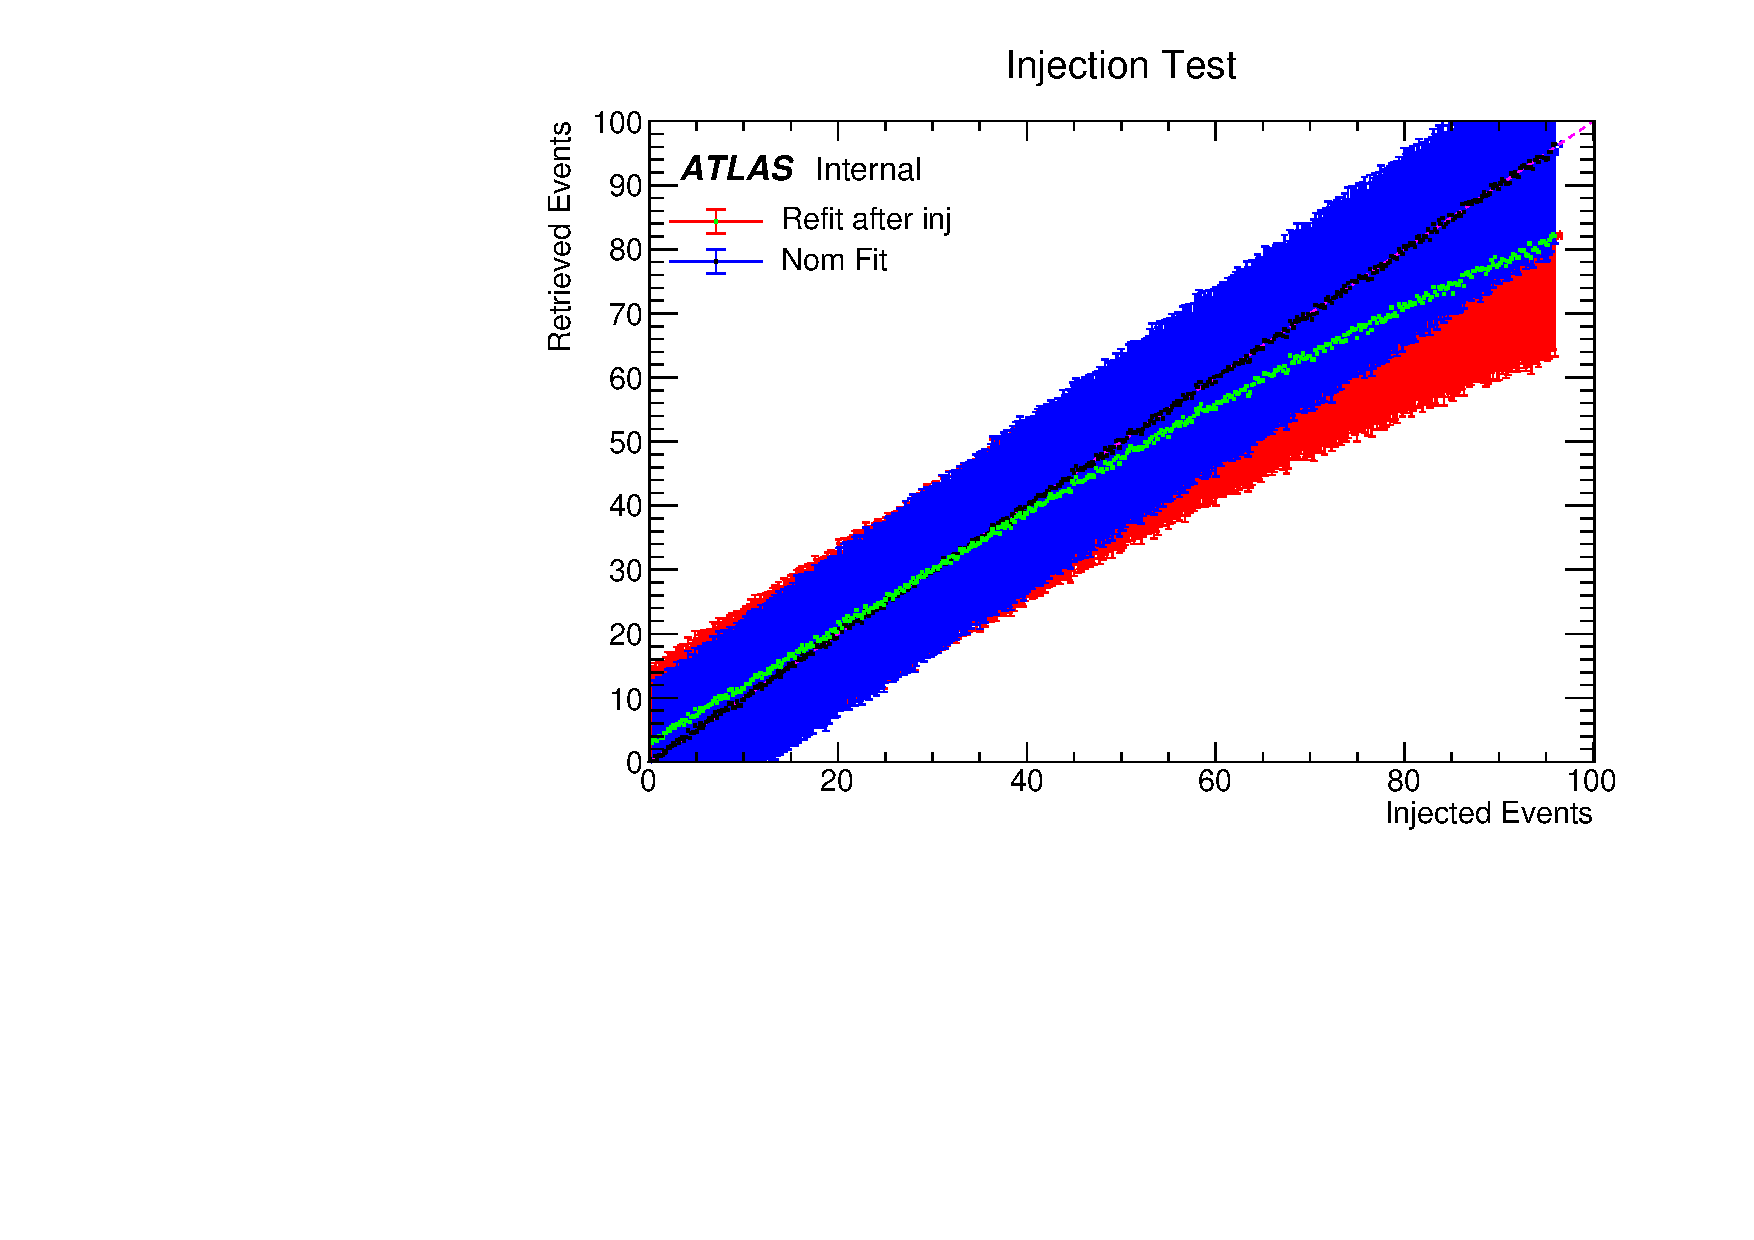
\includegraphics[trim={0cm 0cm 1.6cm 1cm},clip,width=1.0\linewidth]{figures/app-GlobalFitStability/injectionFitStabilityStringScale7000.pdf}
    \caption{Signal stability for a signal injection of a String sample with String Scale 7.0 TeV}
    \label{fig:StringSignalInjectionFitStabilityStudyMs7.0TeV}
\end{figure}
\begin{figure}
    \centering
    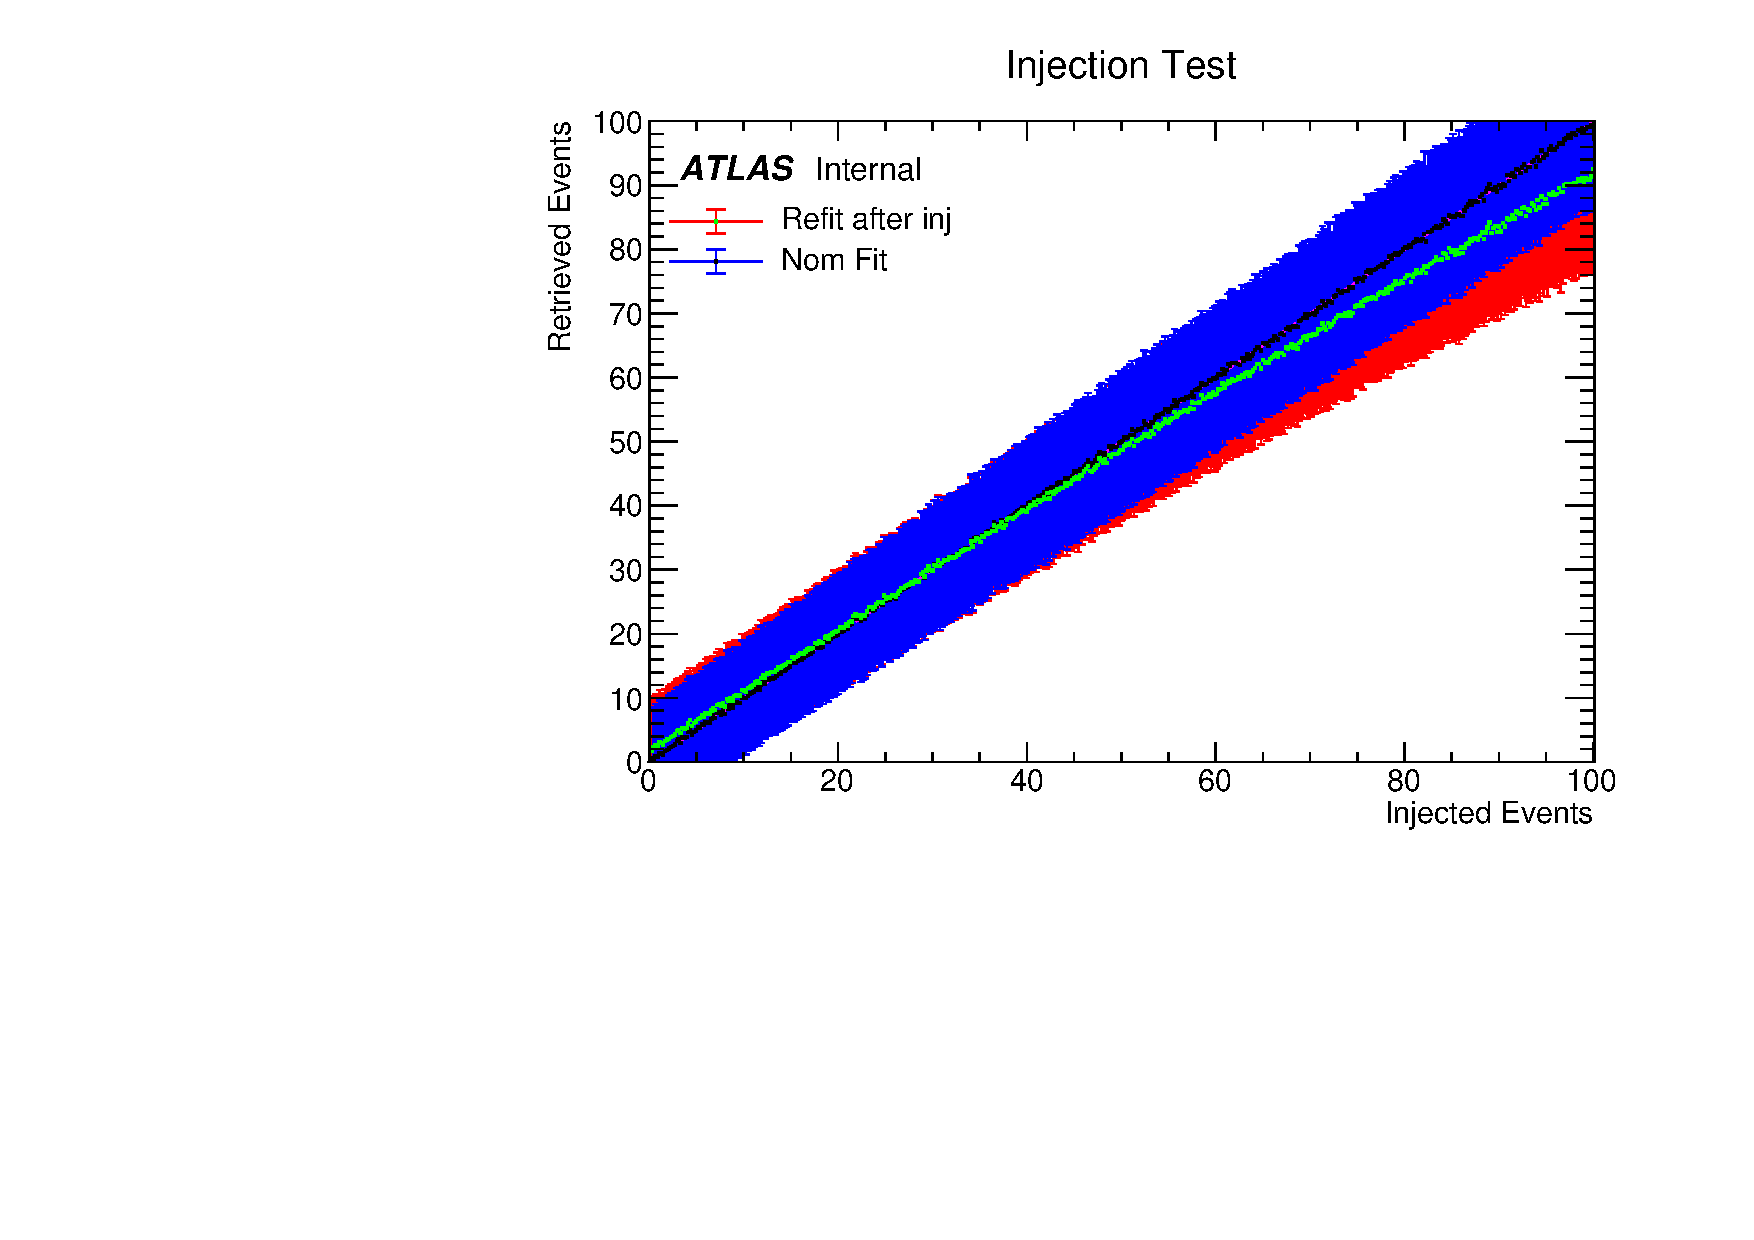
\includegraphics[trim={0cm 0cm 1.6cm 1cm},clip,width=1.0\linewidth]{figures/app-GlobalFitStability/injectionFitStabilityStringScale7500.pdf}
    \caption{Signal stability for a signal injection of a String sample with String Scale 7.5 TeV}
%    \label{fig:StringSignalInjectionFitStabilityStudyMs7.5TeV} % uncomment if label used. 
\end{figure}
\begin{figure}
    \centering
    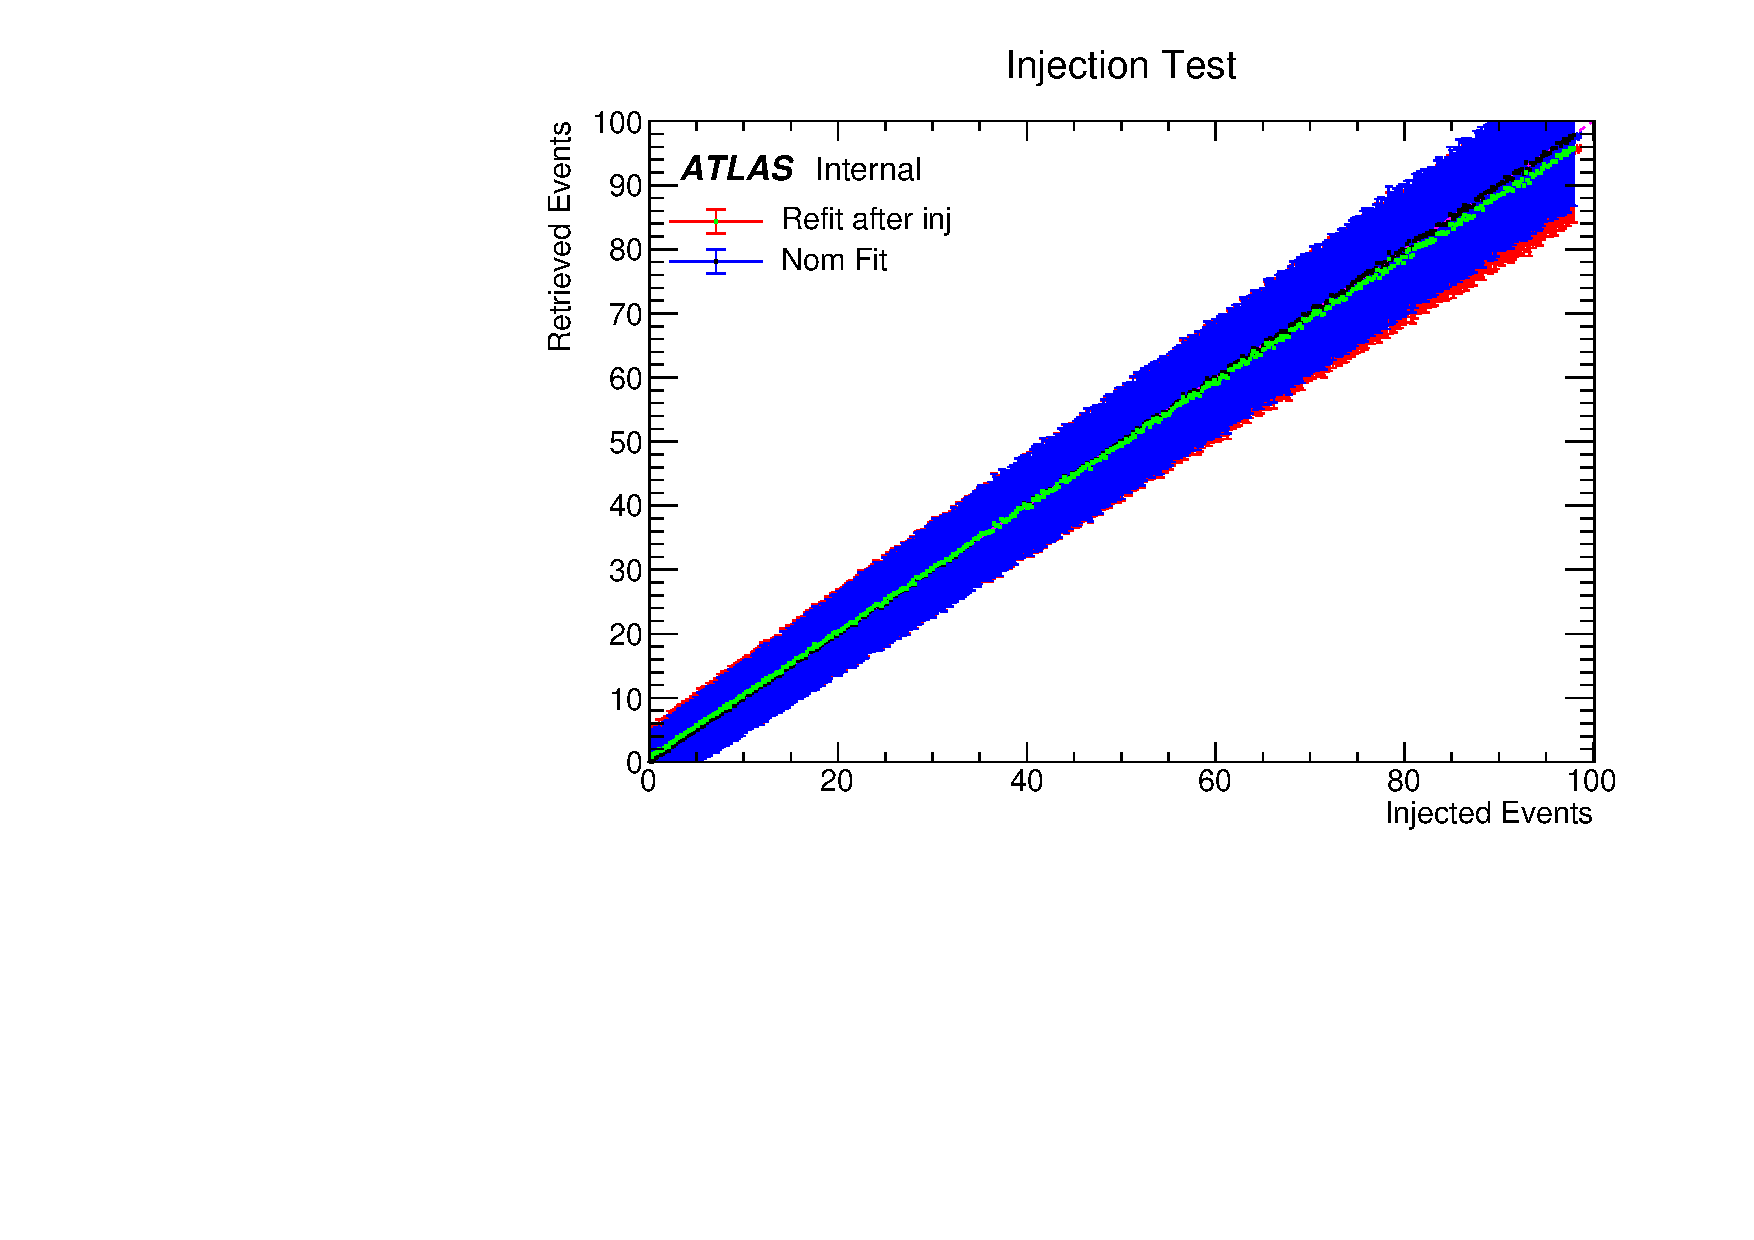
\includegraphics[trim={0cm 0cm 1.6cm 1cm},clip,width=1.0\linewidth]{figures/app-GlobalFitStability/injectionFitStabilityStringScale8000.pdf}
    \caption{Signal stability for a signal injection of a String sample with String Scale 8.0 TeV}
%    \label{fig:StringSignalInjectionFitStabilityStudyMs8.0TeV} % uncomment if label used. 
\end{figure}
\begin{figure}
    \centering
    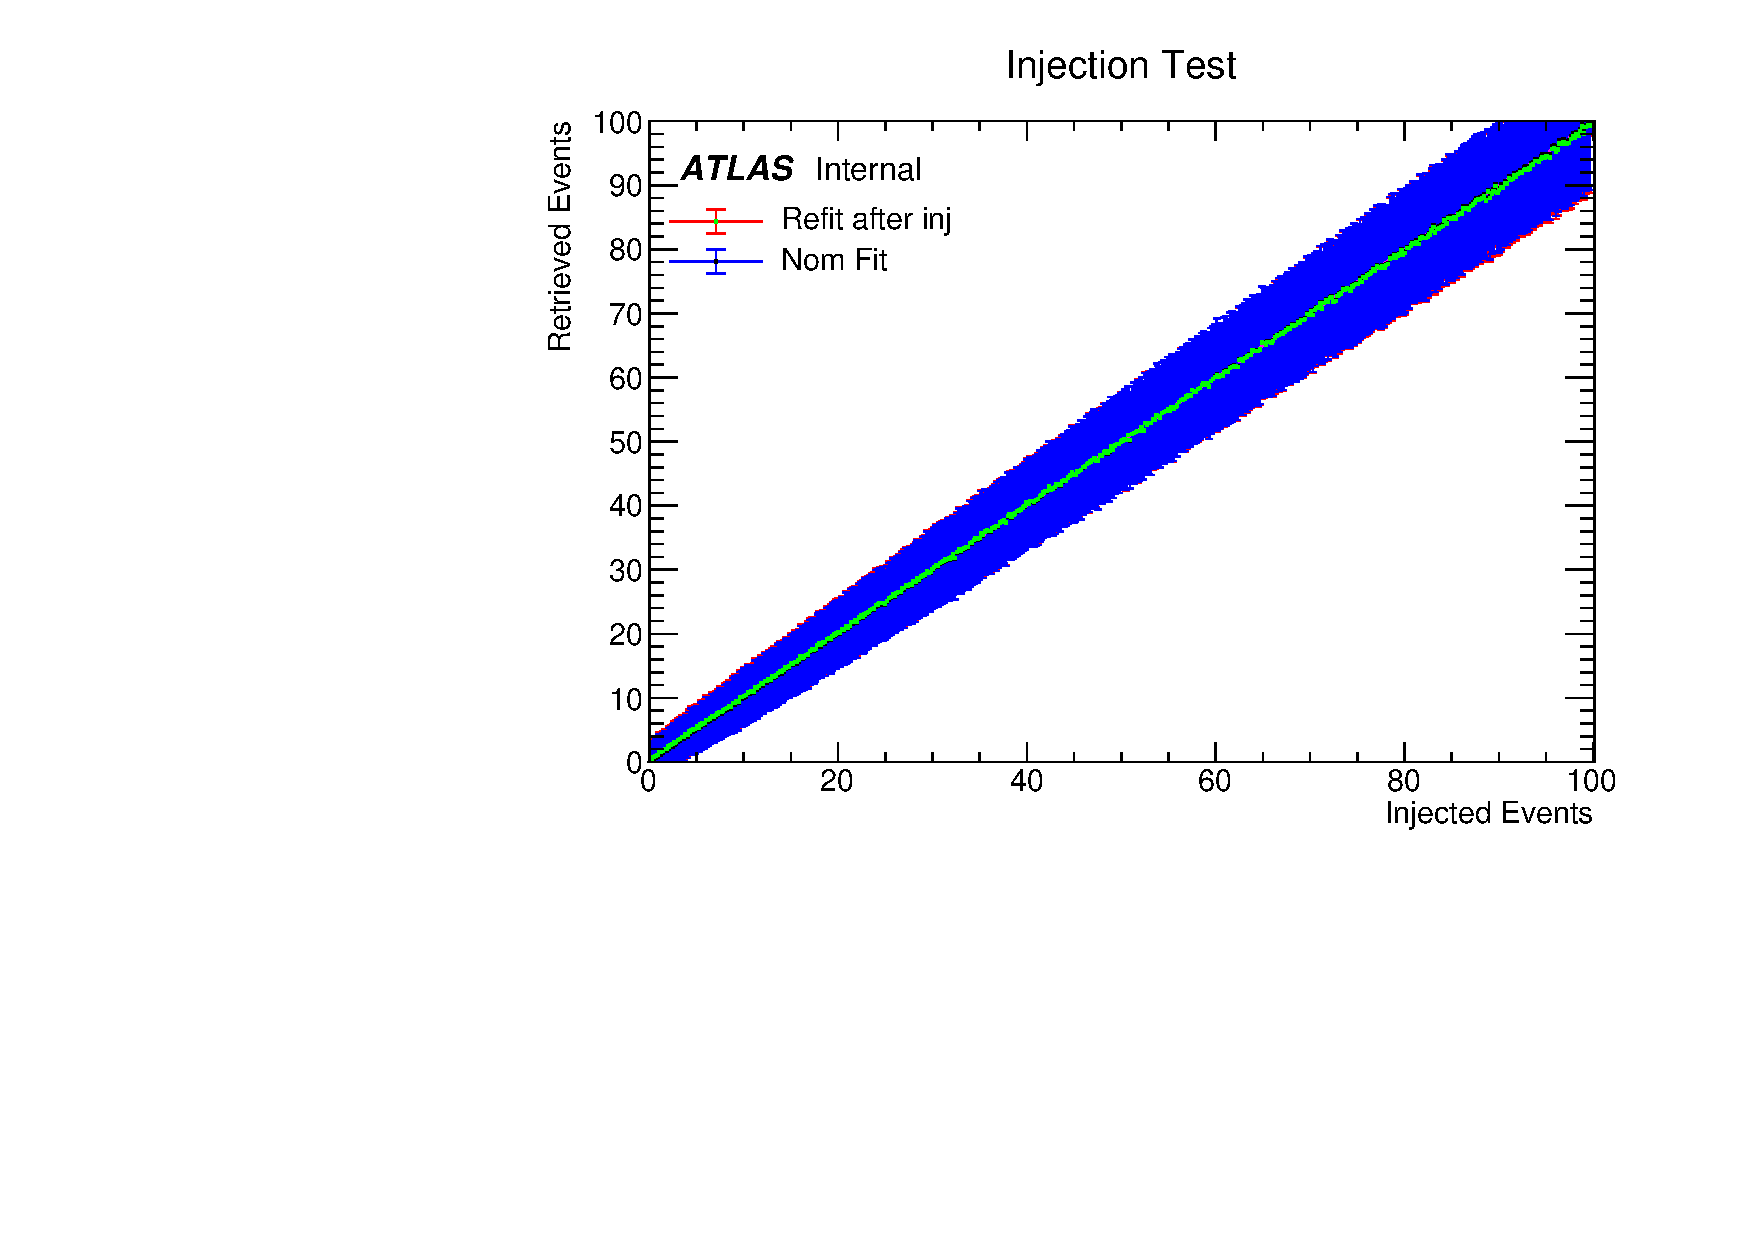
\includegraphics[trim={0cm 0cm 1.6cm 1cm},clip,width=1.0\linewidth]{figures/app-GlobalFitStability/injectionFitStabilityStringScale8500.pdf}
    \caption{Signal stability for a signal injection of a String sample with String Scale 8.5 TeV}
%    \label{fig:StringSignalInjectionFitStabilityStudyMs8.5TeV} % uncomment if label used. 
\end{figure}
\begin{figure}
    \centering
    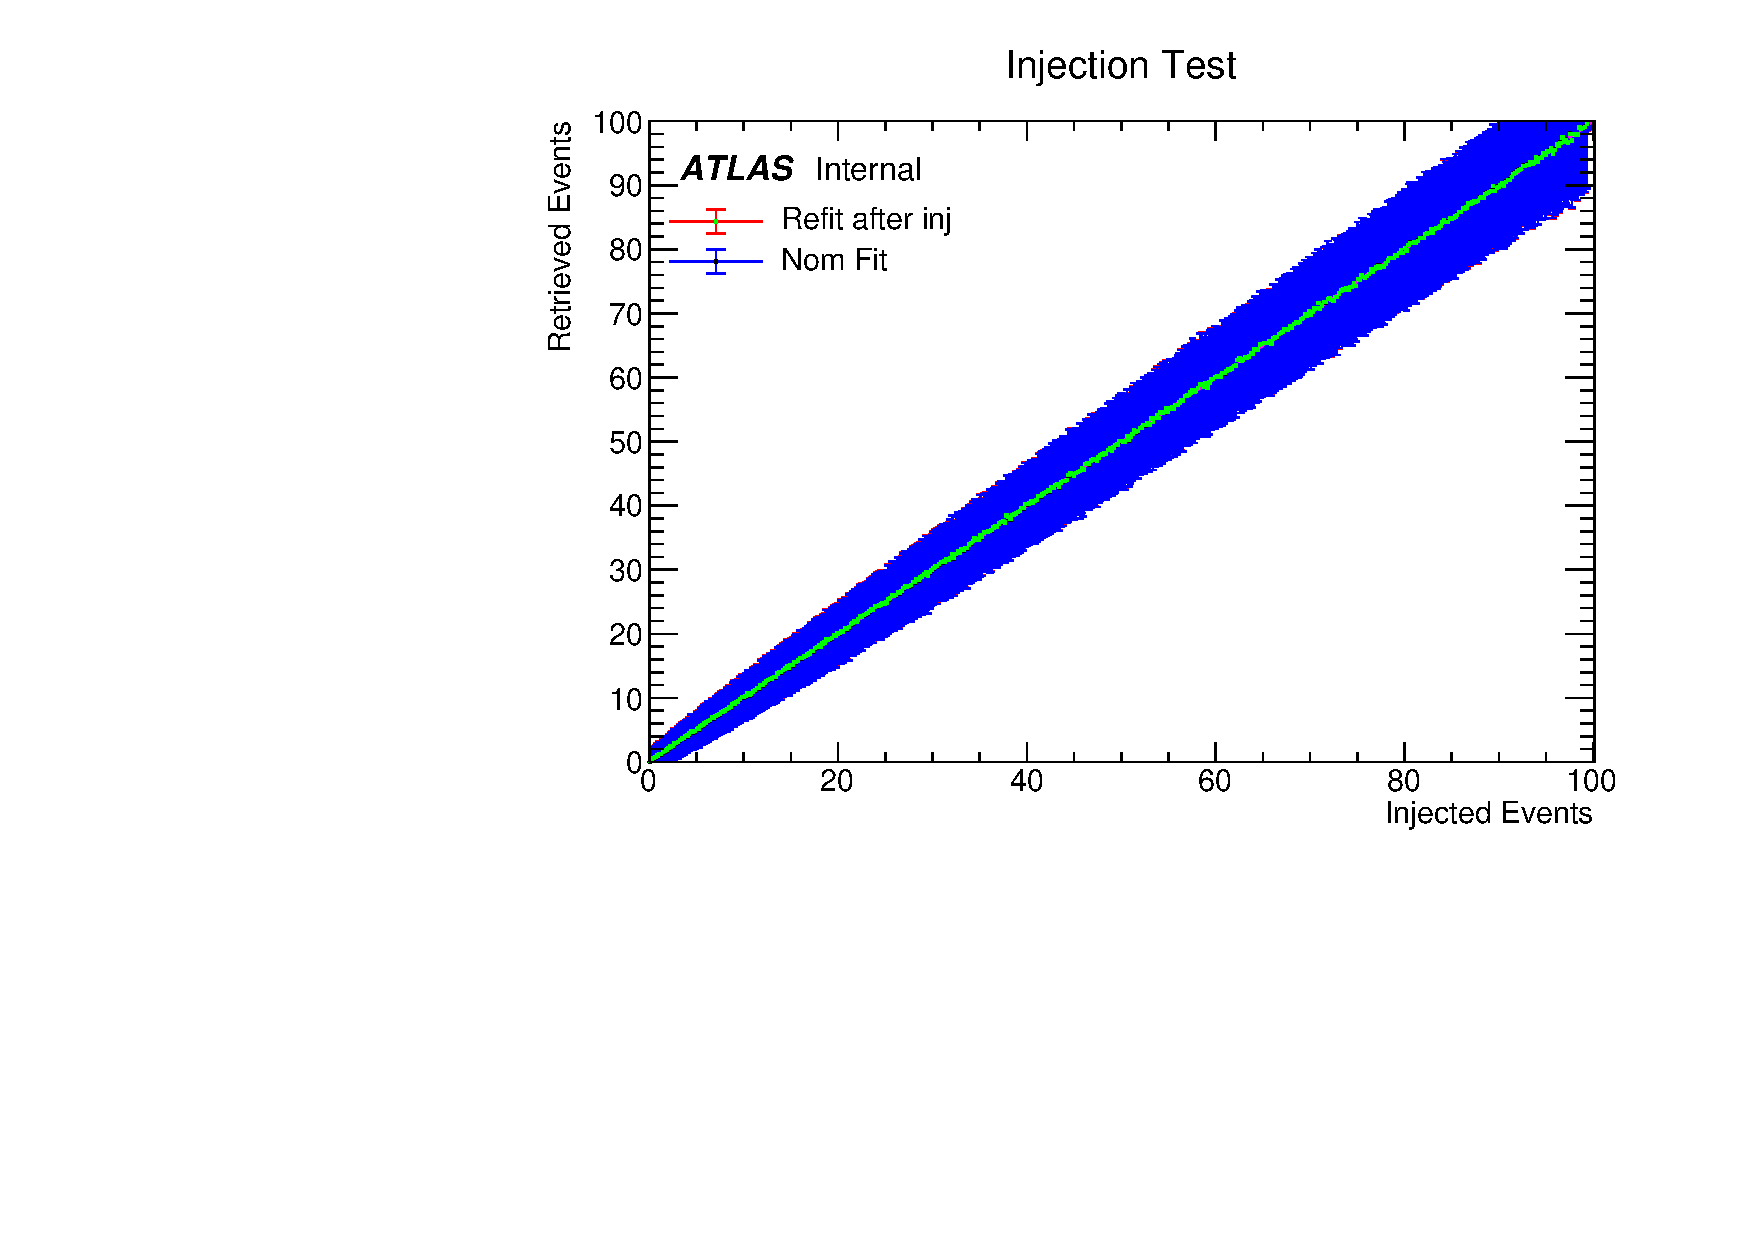
\includegraphics[trim={0cm 0cm 1.6cm 1cm},clip,width=1.0\linewidth]{figures/app-GlobalFitStability/injectionFitStabilityStringScale9000.pdf}
    \caption{Signal stability for a signal injection of a String sample with String Scale 9.0 TeV}
    \label{fig:StringSignalInjectionFitStabilityStudyMs9.0TeV}
\end{figure}

It can be seen that the effect of fit stability upon injection for all String samples investigated is negligible for signals large enough to produce up to and above a BumpHunter significance of 3 $\sigma$. The fit stability is worse (but still negligible) for signals with a resonance at lower $m_{jj}$ for two reasons, being that the effect is larger for a higher number of injected events while at lower $m_{jj}$ more events are needed to be injected to produce a significant signal, and also that for the same number of injected events the effect is larger at lower $m_{jj}$.

\subsection{Spurious Signal}
%\label{subsec:globalFitStability:SpuriousSignal} % uncomment if label used. 

In addition to fit stability under signal injection as investigated in the previous section, it is important to verify that the fit is stable under no signal injection, i.e. that on average the number of retrieved events is consistent with 0. This has been investigated using the same method as the previous section, but instead injecting 0 signal. Then, the number of retrieved events within a region of 0.1 TeV and 1 TeV is measured, to determine that the fit is stable under no signal injection both in a small region and wide region.

The results of this spurious signal fit stability test are shown in Figures \ref{fig:SpuriousSignalInjectionFitStabilityStudy0.1TeVRegion} and \ref{fig:SpuriousSignalInjectionFitStabilityStudy1.0TeVRegion} for the 0.1 TeV and 1 TeV region respectively. It can be seen that the number of retrieved events is consistent with 0 in both cases all across the $m_{jj}$ range. Discontinuity/non-smoothness at very low $m_{jj}$ is purely because of the region investigated going below the minimum $m_{jj}$ cut.

\begin{figure}
    \centering
    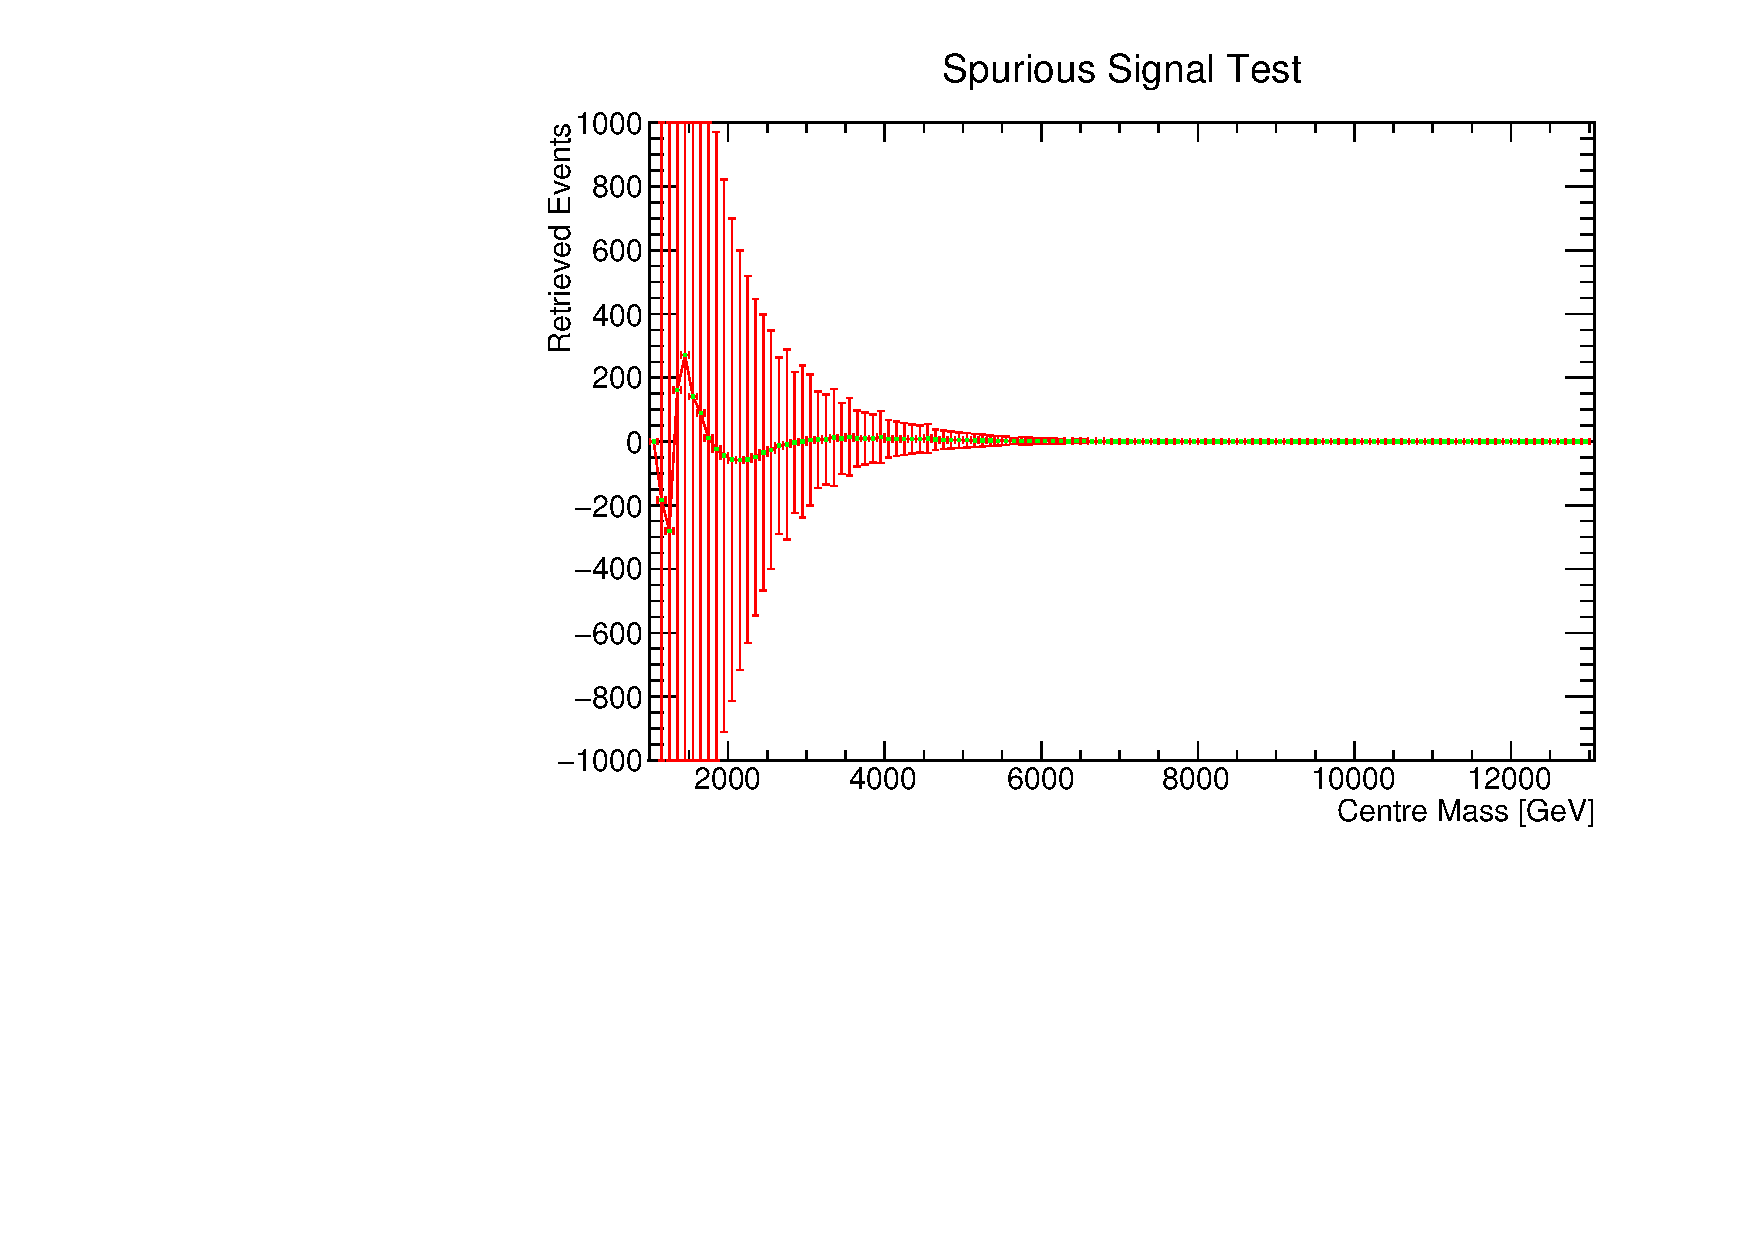
\includegraphics[trim={0cm 0cm 2cm 1cm},clip,width=1.0\linewidth]{figures/app-GlobalFitStability/spuriousSignalFitStabilityWidth100.pdf}
    \caption{Signal stability for no injected signal looking at a region of width 0.1 TeV}
    \label{fig:SpuriousSignalInjectionFitStabilityStudy0.1TeVRegion}
\end{figure}
\begin{figure}
    \centering
    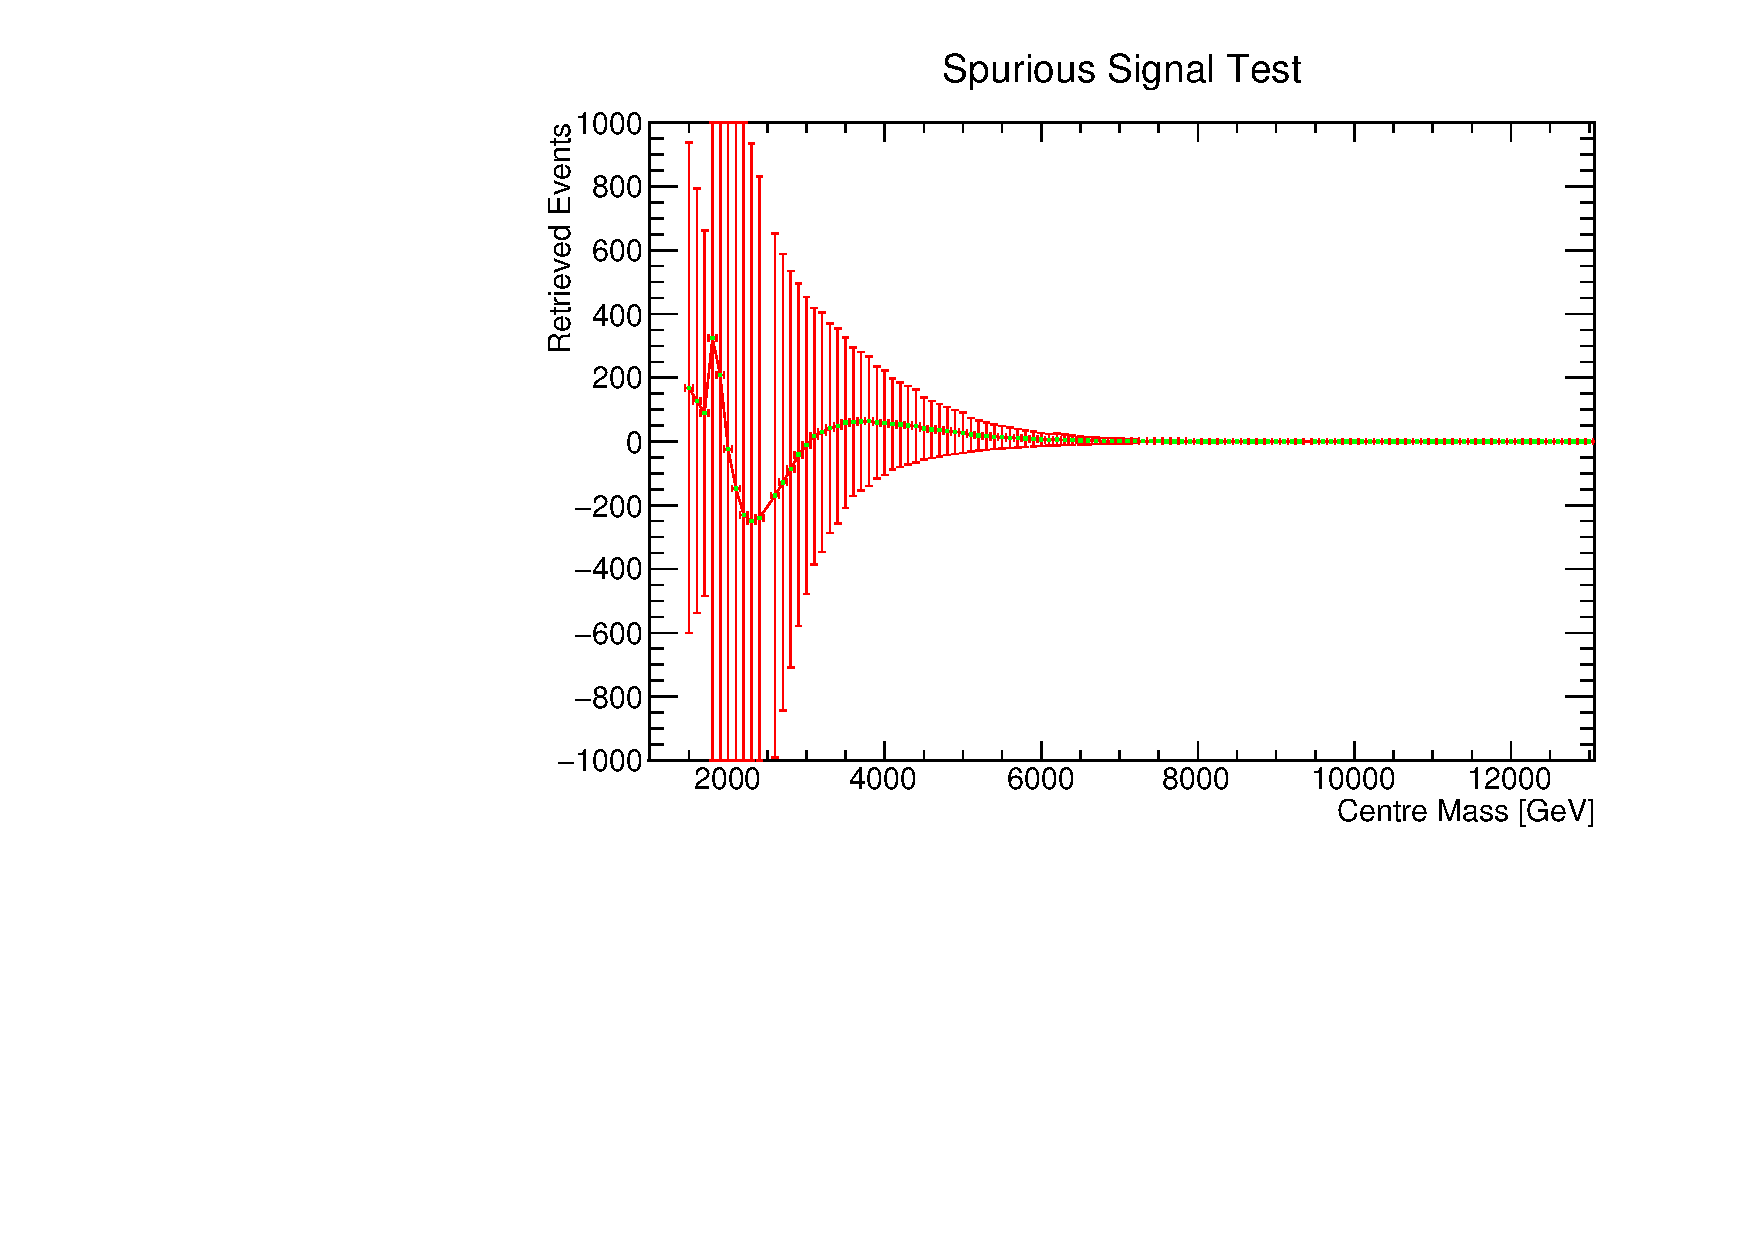
\includegraphics[trim={0cm 0cm 2cm 1cm},clip,width=1.0\linewidth]{figures/app-GlobalFitStability/spuriousSignalFitStabilityWidth1000.pdf}
    \caption{Signal stability for no injected signal looking at a region of width 1.0 TeV}
    \label{fig:SpuriousSignalInjectionFitStabilityStudy1.0TeVRegion}
\end{figure}
